%%
%% This is file `sample-sigconf.tex',
%% generated with the docstrip utility.
%%
%% The original source files were:
%%
%% samples.dtx  (with options: `sigconf')
%% 
%% IMPORTANT NOTICE:
%% 
%% For the copyright see the source file.
%% 
%% Any modified versions of this file must be renamed
%% with new filenames distinct from sample-sigconf.tex.
%% 
%% For distribution of the original source see the terms
%% for copying and modification in the file samples.dtx.
%% 
%% This generated file may be distributed as long as the
%% original source files, as listed above, are part of the
%% same distribution. (The sources need not necessarily be
%% in the same archive or directory.)
%%
%% The first command in your LaTeX source must be the \documentclass command.
\documentclass[manuscript,screen]{acmart}
%% NOTE that a single column version may be required for 
%% submission and peer review. This can be done by changing
%% the \doucmentclass[...]{acmart} in this template to 
%% \documentclass[manuscript,screen]{acmart}
%% 
%% To ensure 100% compatibility, please check the white list of
%% approved LaTeX packages to be used with the Master Article Template at
%% https://www.acm.org/publications/taps/whitelist-of-latex-packages 
%% before creating your document. The white list page provides 
%% information on how to submit additional LaTeX packages for 
%% review and adoption.
%% Fonts used in the template cannot be substituted; margin 
%% adjustments are not allowed.
%%
%%
%% \BibTeX command to typeset BibTeX logo in the docs
\AtBeginDocument{%
  \providecommand\BibTeX{{%
    \normalfont B\kern-0.5em{\scshape i\kern-0.25em b}\kern-0.8em\TeX}}}

%% CUSTOM PACKAGES
\usepackage{multirow}
\usepackage{subcaption}

%% CUSTOM CODE
\usepackage[compact]{titlesec}         % you need this package
\titlespacing{\section}{0pt}{0pt}{0pt} % this reduces space between (sub)sections to 0pt, for example
\AtBeginDocument{%                     % this will reduce spaces between parts (above and below) of texts within a (sub)section to 0pt, for example - like between an 'eqnarray' and text
  \setlength\abovedisplayskip{0pt}
  \setlength\belowdisplayskip{0pt}}

\usepackage[rawfloats=true]{floatrow} 
\restylefloat{figure}     % this, I think, will reduce spaces between images and text.  

% \vspace{-3mm}

%% Rights management information.  This information is sent to you
%% when you complete the rights form.  These commands have SAMPLE
%% values in them; it is your responsibility as an author to replace
%% the commands and values with those provided to you when you
%% complete the rights form.
\setcopyright{acmcopyright}
\copyrightyear{2022}
\acmYear{2022}
\acmDOI{XXXXXXX.XXXXXXX}

%% These commands are for a PROCEEDINGS abstract or paper.
\acmConference[ICCMS '22]{}{June 24--26, 2022}{Chongqing, China}
%
%  Uncomment \acmBooktitle if th title of the proceedings is different
%  from ``Proceedings of ...''!
%
\acmBooktitle{Chongqing '22: 4th International Conference on Computer Modeling and Simulation, June 24--26, 2022, Chongqing, China} 
% \acmPrice{15.00}
% \acmISBN{978-1-4503-XXXX-X/22/06}

%%
%% Submission ID.
%% Use this when submitting an article to a sponsored event. You'll
%% receive a unique submission ID from the organizers
%% of the event, and this ID should be used as the parameter to this command.
%%\acmSubmissionID{123-A56-BU3}

%%
%% The majority of ACM publications use numbered citations and
%% references.  The command \citestyle{authoryear} switches to the
%% "author year" style.
%%
%% If you are preparing content for an event
%% sponsored by ACM SIGGRAPH, you must use the "author year" style of
%% citations and references.
%% Uncommenting
%% the next command will enable that style.
%%\citestyle{acmauthoryear}

%%
%% end of the preamble, start of the body of the document source.
\begin{document}

%%
%% The "title" command has an optional parameter,
%% allowing the author to define a "short title" to be used in page headers.
\title{Dynamic models for analysing stock market behaviour under the COVID-19 pandemic}

%%
%% The "author" command and its associated commands are used to define
%% the authors and their affiliations.
%% Of note is the shared affiliation of the first two authors, and the
%% "authornote" and "authornotemark" commands
%% used to denote shared contribution to the research.
\author{Maarten Peters}
% \authornote{Main author}
\email{maarten.peters@gmail.com}
\affiliation{%
  \institution{University of Amsterdam}
  \streetaddress{Science Park 904}
  \city{Amsterdam}
  % \state{Ohio}
  \country{the Netherlands}
  \postcode{1098 XH}
}

\author{Dr. Cristian Rodriguez Rivero}
\authornote{Internal Supervisor from the University of Amsterdam as part of the master thesis programme}
\email{c.m.rodriguezrivero@uva.nl}
\affiliation{%
  \institution{University of Amsterdam, FNWI, IvI}
  \streetaddress{Science Park 904}
  \city{Amsterdam}
  % \state{Ohio}
  \country{the Netherlands}
  \postcode{1098 XH}
}

\author{Dr. Julián Antonio Pucheta}
\authornote{External Supervisor from the National University of Córdoba}
\email{jpucheta@unc.edu.ar}
\affiliation{%
  \institution{Universidad Nacional de Córdoba}
  \streetaddress{Av. Haya de la Torre}
  \city{Córdoba}
  % \state{Ohio}
  \country{Argentina}
  \postcode{HR77+RQ}
}

%%
%% By default, the full list of authors will be used in the page
%% headers. Often, this list is too long, and will overlap
%% other information printed in the page headers. This command allows
%% the author to define a more concise list
%% of authors' names for this purpose.
\renewcommand{\shortauthors}{Maarten Peters, et al.}

%%
%% The abstract is a short summary of the work to be presented in the
%% article.
\begin{abstract}
During the COVID-19 pandemic \cite{velavan2020covid} questions were raised on how to balance government measures ensuring population health and allowing economic development. At the start of the pandemic, Saudi-Arabia and Russia were in a pricing war over crude oil \cite{jacobs2020opec} which, along with speculation on the economic impact of COVID-19, led to a unprecedented negative crude oil price in the West Texas Intermediate (WTI) \cite{CORBET2020104978}. As the WTI serves as a benchmark for crude oil prices in North America, and a proxy for economic development \cite{kaufmann2011role}, it is an interesting candidate to use for price forecasting \cite{YU20082623}. The pandemic provides a unique perspective, as it introduces a new set of variables \cite{dong2020interactive, hale2020variation}, such as infections, deaths, vaccinations and government measures \footnote{Provided by the National Institute for Public Health and the Environment (in Dutch: Rijksinstituut voor Volksgezondheid en Milieu, RIVM), the Johns Hopkins University Coronavirus Resource Center (JHU) and the Oxford COVID-19 Government Response Tracker (OxCGRT).}, that might aid in predicting economic development \cite{chudik2020economic, baldwin2020economics, fernandes2020economic}. Related studies generally focus on macroeconomic development, such as gross domestic product (GDP), unemployment or inflation over years or decades, rather than short-term development over days, weeks or months. This study attempts to combine data from the COVID-19 pandemic, weather, stock pricing data and machine learning techniques to determine the relationship between these variables and their value towards more accurate price forecasting. As stock prices have high variance, extreme values might indicate local or global stock market crashes, an optimal model would be able to predict these crashes. To determine the outcome of our research question, we compare the value of our data between a baseline model, linear model and two state-of-the-art (SOTA) models, the random forest regressor (RFR) and auto-regressive integrated moving average (ARIMA) model. Both SOTA models tend to perform better or similar with less features, indicating the data does not add significant value to the prediction of stock market values.
\end{abstract}

%%
%% The code below is generated by the tool at http://dl.acm.org/ccs.cfm.
%% Please copy and paste the code instead of the example below.
%%
%%\begin{CCSXML}
%%<ccs2012>
 %%<concept>
%%  <concept_id>10010520.10010553.10010562</concept_id>
%%  <concept_desc>Computer systems organization~Embedded systems</concept_desc>
%%  <concept_significance>500</concept_significance>
 %%</concept>
 %%<concept>
%%  <concept_id>10010520.10010575.10010755</concept_id>
%%  <concept_desc>Computer systems organization~Redundancy</concept_desc>
%%  <concept_significance>300</concept_significance>
 %%</concept>
 %%<concept>
%%  <concept_id>10010520.10010553.10010554</concept_id>
%%  <concept_desc>Computer systems organization~Robotics</concept_desc>
%%  <concept_significance>100</concept_significance>
 %%</concept>
 %%<concept>
%%  <concept_id>10003033.10003083.10003095</concept_id>
%%  <concept_desc>Networks~Network reliability</concept_desc>
%%  <concept_significance>100</concept_significance>
 %%</concept>
%%</ccs2012>
%%\end{CCSXML}
%%
%%\ccsdesc[500]{Computer systems organization~Embedded systems}
%%\ccsdesc[300]{Computer systems organization~Redundancy}
%%\ccsdesc{Computer systems organization~Robotics}
%%\ccsdesc[100]{Networks~Network reliability}

\begin{CCSXML}
<ccs2012>
   <concept>
       <concept_id>10010147.10010257.10010293.10010307</concept_id>
       <concept_desc>Computing methodologies~Learning linear models</concept_desc>
       <concept_significance>300</concept_significance>
       </concept>
 </ccs2012>
\end{CCSXML}

\ccsdesc[300]{Computing methodologies~Learning linear models}

%%
%% Keywords. The author(s) should pick words that accurately describe
%% the work being presented. Separate the keywords with commas.
\keywords{COVID-19, dynamic processes, stock market index, multivariable analysis, time series forecasting}

%% A "teaser" image appears between the author and affiliation
%% information and the body of the document, and typically spans the
%% page.
% \begin{teaserfigure}
%   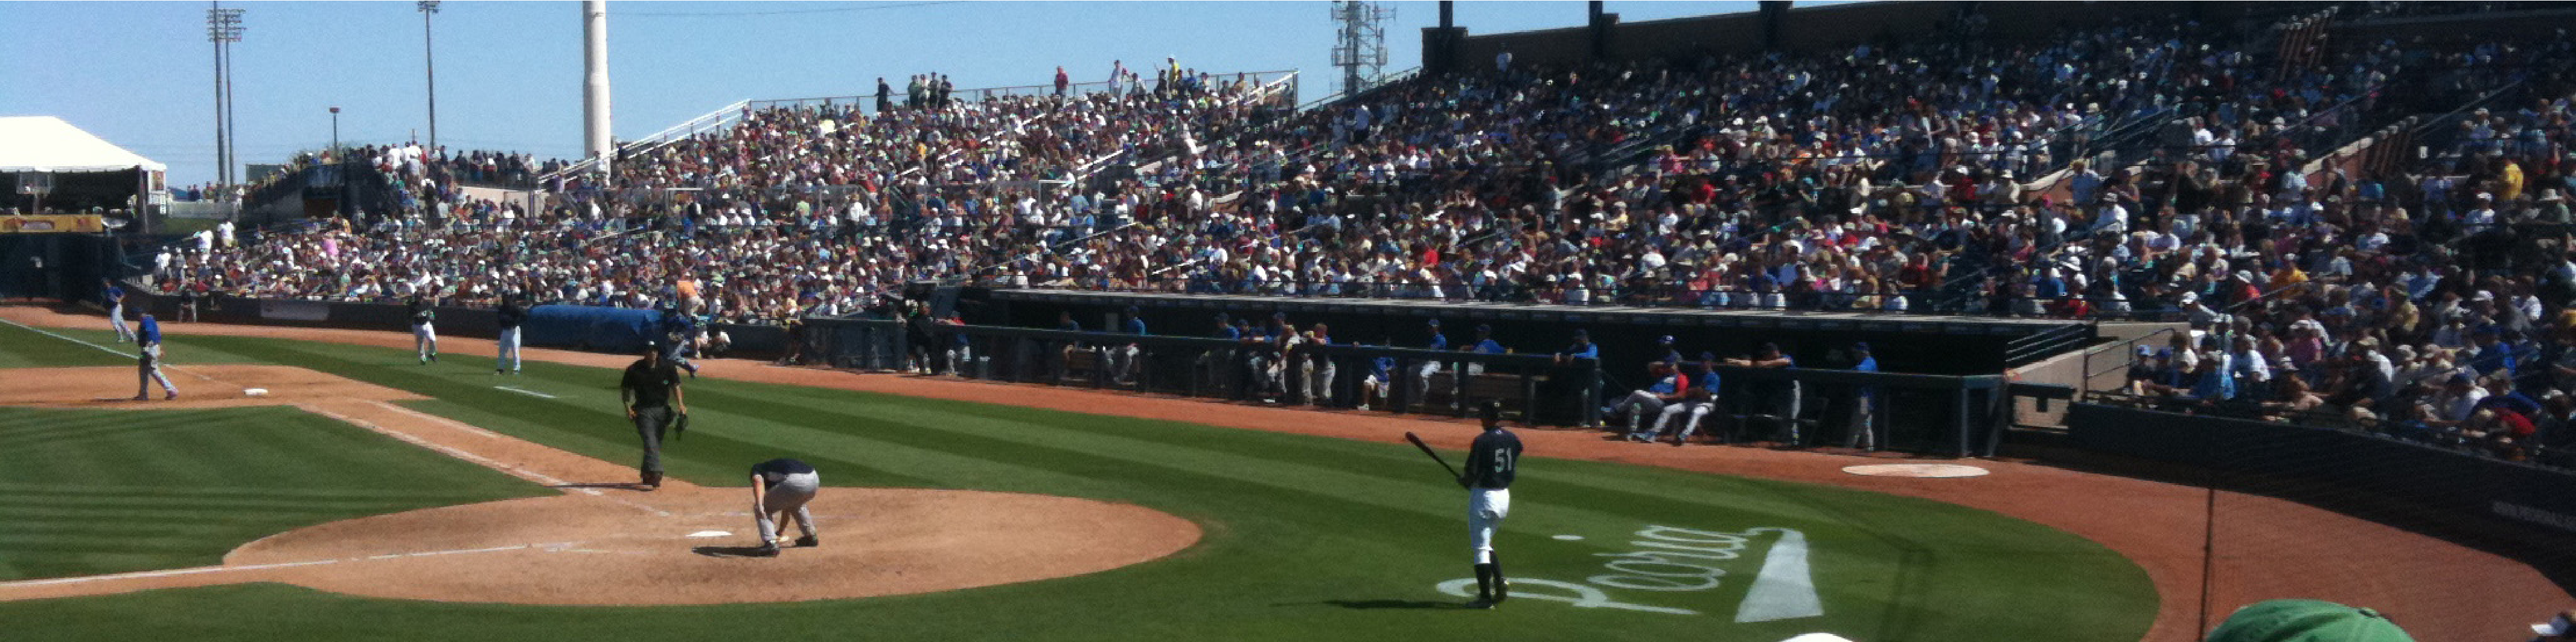
\includegraphics[width=\textwidth]{sampleteaser}
%   \caption{Seattle Mariners at Spring Training, 2010.}
%   \Description{Enjoying the baseball game from the third-base
%   seats. Ichiro Suzuki preparing to bat.}
%   \label{fig:teaser}
% \end{teaserfigure}

%%
%% This command processes the author and affiliation and title
%% information and builds the first part of the formatted document.
\maketitle

\section{Introduction}
\label{sec:intro}
At the start and during the COVID-19 pandemic, rising infection rates, deaths and widespread lockdown measures raised questions on how to limit the pandemic's impact on economic development \cite{velavan2020covid}. This thesis looks into how the pandemic affects stock market values, as these are notoriously volatile in their pricing and influenced by a wide range of factors, demonstrated by the WTI value dipping in the negative at the first wave of infections \cite{CORBET2020104978}. 
The relationship between stock markets and economic factors falls under the study of macroeconomics and finds it origins in the business cycle theory, dating back to the early 1800s \cite{de1827nouveaux}. This theory generally states that all economic development follows a cycle or waveform, going through the phases expansion, crisis, recession and recovery. These business cycles can be measured \cite{baxter1999measuring} and are part of the tools that a government can use to mitigate economic downturn. Predicting the development of a business cycle is generally based on economic indicators and economic theory, such as Keynesian theory  \cite{keynes2018general} and real-business cycle (RBC) theory \cite{kydland1982time}. One of the generally accepted economic indicators is the Standard and Poor's (S\&P) 500 as an indicator for the United States (US) economy, stating a relationship between economic development and the top 500 US companies. % \cite{diblasi_2021}
One of the complexities of these relationships, between a country and a national representation of the local stock market, is that a stock market is not a local phenomenon. Stocks and other financial products are traded internationally via a stock exchange and these stock indexes, such as the S\&P500, are a representation of the stock exchange itself and not (necessarily) of the country it resides in. As the pandemic's impact and government restrictions varies between countries, it is needed to isolate a region to perform a causal analysis of its impact on a stock market.
When the WTI value dropped, all oil-related stocks dropped in value as a consequence, such as Royal Dutch Shell, one of the largest companies in the Netherlands. As previous research noted a relationship between pandemic data and economic development, and a relationship between economic development and stock indexes, the question can be posed whether these relationships aid in predictive modelling of stock values in a region. This research will focus on the Netherlands, with the Amsterdam Exchange index (AEX) as an analog for the S\&P500, the former featuring the top 25 most traded securities on the Amsterdam Exchange. As macroeconomics looks at the large scale development of an economy, the models generally apply to years or decades of data. Daily stock market development is a lot more volatile than other economic indicators, generally displaying a non-linear patterns. 
Machine learning can aid in these predictions, as it can capture non-linear behaviour better than traditional linear models \cite{zhang2009stock}. Still, stock market prediction is non-trivial as the efficient market hypothesis (EMH) \cite{peters1996chaos} states that no investor can gain an advantage over others based on historical and current information. Some investors base their decisions on fundamental analysis \cite{lev1993fundamental} to gain an advantage on others. Machine learning has shown to be effective at improving prediction accuracy on stock market securities or crude oil pricing \cite{jain1996, YU20082623, zhang2009stock, thawornwong2004forecasting}, especially using recurrent- (RNN) or artificial neural networks (ANN). % \cite{crotty2009} \cite{garber1989}
Having established the relationship between stock market values and economic development, the question remains whether the pandemic actually influenced stock market values. Social and economic factors have shown historical importance in stock market crashes, such as with the Tulip Mania, the Wall Street Crash of 1929 and the Great Depression \cite{white1990, kindleberger1986world} and the global financial crisis of 2008. An important topic during the recent pandemic was whether it would influence the economy and what its impact would be. Historically pandemics have shown their effects \cite{osterholm2017preparing, correia1918pandemics, jorda2020longer}, but the quantitative relationship between the COVID-19 pandemic and economic development is still an object of research \cite{chudik2020economic, baldwin2020economics, fernandes2020economic, deb2020economic}. During the pandemic daily data was registered on its development, such as infection rates, deaths, vaccinations and government restrictions \cite{dong2020interactive, hale2020variation}. As stock market crashes generally are a social phenomenon, this research investigates the relationship between these features and stock market pricing. The following research questions are posed:
\begin{itemize}
    \item[RQ1] \ldots To what extent does the COVID-19 pandemic data influence stock market values?
        \begin{itemize}
            \item What is the baseline performance for standard statistical models on short term and long term?
            \item How do different statistical and machine learning models compare given the same data?
            \item How do models generalize to different time-periods, such as distinctions between different infection waves?
            \item Which variables in a pandemic affect stock market pricing and to what extent? % Variables such as ...
            % \begin{itemize}
            %     \item COVID-19 pandemic data incl.: infections, deaths, vaccinations and % government restrictions
            %     \item Environmental factors such as calendar data or weather
            % \end{itemize}
        \end{itemize}
    \item[RQ2] \ldots To what extent can machine learning techniques aid in predicting stock market pricing, given a comparison of baseline models and the addition of pandemic data?
\end{itemize}
As the pandemic influenced a wide array of human behaviours, variables are restricted to the ones mentioned above. Other variables, such as mobility, energy consumption and social contacts have shown large differences during the pandemic, but are outside of the scope of this research.
% \paragraph{Overview of paper}
% To create context and support of the hypothesis, this paper first discusses related work \ref{sec:rel}. With this context, a proper methodology \ref{sec:meth} is formulated with an explanation on the data collection \ref{sec:data}, model development \ref{sec:models} and how these answer the proposed research questions \ref{sec:eval}. Using the methodology and proper context from related work, results can be analysed \ref{sec:res}, discussed \ref{sec:dis} and be made to construct a conclusion \ref{sec:conc}.
\section{Related Work}
\label{sec:rel}
% As this paper looks at the influence of COVID-19 pandemic data on stock market values, a couple of sections are dedicated to discuss related work. As the research questions are related to models and data, these are discussed as separate topics.
\subsection{Data}
\subsubsection{Pandemic Data}
As the COVID-19 pandemic began to increase in number of cases, world-wide spread and severity, a large part of the academic world focused their efforts on solving issues related to the pandemic or contributing to the cause in general. One of the most influential parties was the Johns Hopkins University's (JHU) with their Coronavirus Research Center (CRC) and their Center for Systems Science and Engineering (CSSE) \cite{dong2020interactive}. They started one of the first and most successful data collections around the COVID-19 pandemic and provided world-wide figures into the number of infections, deceased and (in a later stage) vaccinations, for varying degrees of granularity. In the early stages of the pandemic, the focus was much more regional \cite{HUANG2020497, wang2020novel, velavan2020covid} and built around statistics such as reproductive numbers, health effects and possible treatments. As the effects of COVID-19 on the community became more apparent and the severity of the pandemic increased, governments became concerned on its effect on society and if their could be economic consequences.
It became clear that lockdown measures were necessary to reduce the number of infections. The exact measures differed from country to country, as the effectiveness of measures were always a matter of debate. Societal measures ranged from curfews mandating people to stay at home and reduce non-essential traveling, mandatory social distancing assuring people refrain from physical contact \cite{lewnard2020scientific} or the wearing of face masks in public spaces to reduce the spread of airborne viral particles \cite{eikenberry2020}. Businesses also faced several restrictions, as the hospitality and tourism industries were forced to close, as they could become hot-spots for disease transmission \cite{gossling2020pandemics}. This in turn also affected the air-travel industry, as people were recommended to stay home and borders were closed off for international travel. And lastly, any other business were often required to provide means for personnel to work remotely from their homes, as offices could also become hot-spots for virus transmission \cite{dingel2020many}. As these measures varied, especially when each country developed infection peaks at different times, there became a need for COVID-19 related research to have a unified way of charting these measures. The Blavatnik School of Government, part of the University of Oxford, provides a centralized dataset that collects and standardizes the measures taken by countries to reduce the effect of the pandemic \cite{hale2020variation}. They provide categories such as containment and closure policies, economic policies, health system policies, vaccination policies and miscellaneous policies over which they proposed a stringency index that indicates the severity of the measures applied.

\subsubsection{Environmental Data}
As this study revolves around effects on stock market data, environmental factors can not be excluded. Although stock market data are very volatile, their variance can be explained as results from human behaviour. And as humans are affected by a variety of physical and psychological effects, these can be attributed to environmental factors, such as weather \cite{hirshleifer2003good}. For example, without going into the principals behind causality, one might argue that there is a causal relationship between sunny weather and ice-cream sales, as people tend to buy more ice-cream during sunny (summer) days. This is an example of human behaviour being influenced by environmental factors, a phenomenon also influencing decisions of traders on the stock market. Still, human behaviour on the stock market can be erratic as people have to deal with uncertainty \cite{tversky1974judgment}. % and can overreact to news \cite{de1985does}.
% With weather data being location bound, publicly available and easily quantifiable, it serves as an ideal candidate for environmental factors in this study. It does come with some caveats, such as it not always being available historically or not being reliable as some data providers rely on community driven data. Another issue is that weather data is localized, as compared to stock market data, which allows international trade. Still an effect might be noticeable and it serves as a good candidate for correlation and hypothesis testing when compared to pandemic data.
Another large factor in stock market data might be stock related news \cite{tversky1974judgment, veronesi1999stock, onsumran2015gold, wang2019internet}. The difficulty of news articles is that they're not easily quantifiable, unless they have been labeled for the specific use case. % Unsupervised machine learning methods can be applied to perform sentiment analysis and topic modelling, but this requires large amounts of data and compute resources with low certainty of added value. Textual data also tends to contain a lot of noise, so it requires extensive cleaning before it can be used appropriately. Therefore this research will forego using stock market related news as input data, as it might interfere with the other variables in the research questions.
Another factor in the research questions is the use of calendar data. As stock markets tend to close during weekends and holidays, this data might aid in identifying seasonal patterns. This research will focus on daily and weekly data, as this is the highest frequency data available for stock markets without the use of paid data providers. Pandemic data is also provided on a daily interval, so this coincides fittingly with the other datasets.

\subsection{Forecasting models}
As the COVID-19 pandemic is a recent phenomenon, studies modelling economic development after the pandemic have been performed but not yet proven \cite{chudik2020economic, baldwin2020economics, fernandes2020economic}. There have been efforts on modelling historic pandemics \cite{osterholm2017preparing, correia1918pandemics, jorda2020longer}, but most of these studies focus on long-term macroeconomic effects, such as gross domestic product (GDP), unemployment, individual/national income, consumption or inflation, looking at years or decades of development. As economic development itself is a slow process, influence by relatively short-term factors such as the stock market is a non-trivial matter. As modern technology provides an unprecedented amount of data for the pandemic \cite{dong2020interactive, hale2020variation}, some research has been done on the short-term development and effects of the pandemic \cite{zhao2020preliminary, deb2020economic, carpi2021twitter}.
A common practice in the development and selection of forecasting models is to perform exploratory data analysis (EDA) and select the model based on an error metric and/or subjective knowledge of the specific domain. Econometric and statistical models generally differ between these disciplines, as the former looks more at domain knowledge and adjusts the model accordingly to reduce error, while the latter relies on statistical methods to reduce model errors. As stock market data is quite volatile, using either of these disciplines can lead to a successful forecasting model, but the theoretical basis differs. As the discipline of data science and machine learning is in essence an evolution of statistics, its methods rely more on error metrics, even though a lot of gains can be made with problem specific model tuning. This study will look solely at the error metrics of models to determine the effectiveness of the model in an automatic manner.
% As a baseline comparison, this study has developed a naive model that assumes no trends or variation in the response variable and forecasts the last known value of a time-series. Given the predictor variable will realistically increase or decrease with every time-step $t$, it is assumed it will always show an error, but it will average out over multiple time-series, given normalized data and a relative error metric.
This study looks into an automatic method of fitting a multiple models, with linear regression and ARIMA as statistical models. The Random Forest Regressor (RFR) represents a precursor of the deep learning \cite{lecun2015deep} field, implemented in a standard Python library\footnote{sklearn: Machine Learning in Python: \url{https://scikit-learn.org/}}. % , goodfellow2016deep

% \subsubsection{Linear model}
% The discipline of forecasting goes back to the early 1700s with the prediction of the return of Halley's comet, where orbital mechanics predicted that the comet returned every 76 years. Decades later mathematicians and physicists Legendre, Gauss and Quetelet developed this theory into the basics of linear regression, the standard for most forecasting problems \cite{stigler1986history}. Linear regression (LR) assumes constant variance, independence of errors and linearity of the data. As the data can be transformed to better fit these characteristics, it has been the basic model for most of econometrics \cite{greene2003econometric}.

% \subsubsection{Random Forest Regressor}
% Statistical models, although occasionally quite complex, can be explained as a mathematical relationship between explanatory and response variables. Machine learning algorithms, although mathematically motivated, tend to be less clear on their inner workings by being a function of the training data. They tend to work in non-linear situations by combining (relatively) simple mathematical models into ensembles, creating a larger non-linear model, forming the basis of a discipline known as deep learning \cite{lecun2015deep, goodfellow2016deep}. Although most machine learning models require a lot of data to be trained, a selection of models has been made available in a Python library to ease machine learning development \footnote{sklearn: Machine Learning in Python: \url{https://scikit-learn.org/}}. One of the models that performs relatively well on small amounts of data is the Random Forest Regressor. A Random Forest is an random ensemble of shallow decision trees, bagged together to create a single model, capable of classification or regression tasks. Properly trained and implemented, they can achieve high accuracy, with the trade-off of lacking interpretability. Where related research implemented neural networks \cite{thawornwong2004forecasting}, these require significant tuning for good performance. Because this study looks at comparing models over a variety of data, this rules out implementing RNNs/ANNs for the sake of generalization.

% \subsubsection{ARIMA} %  \cite{siaminamini2018forecasting, chatfield2019analysis}
% As linear regression can be seen as a basic implementation of regression, the ARIMA model is the most robust regression model that can be used in this context. It also allows for automatic fitting which tries to find an optimal fit by stepping through its parameters \footnote{pmdarima: ARIMA estimators for Python: \url{https://alkaline-ml.com/pmdarima}}, although this might lead to over- or underfitting.
\section{Methodology}
\label{sec:meth}
Given the defined research questions and related work to this study, it needs to adhere to the basic steps of forecasting \cite{hyndman2018forecasting, davydenko2021forecast}: data \ref{sec:data}, models \ref{sec:models} and evaluation \ref{sec:eval}.
To determine the extent of influence of the pandemic on stock market pricing, all factors in the questions are isolated and answered separately. The effect of the data can be determined by using comparisons in correlation scores between features or non-parametric tests. This gives a reliable result for one-on-one relationships between explanatory and response variables, but this becomes a lot more complex in multivariate analysis. This study proposes an alternative solution by comparing forecasting performance using a dynamic model framework where feature importance is compared by applying the mean absolute percentage error (MAPE) on a selection of machine learning models, isolating features between comparisons. $$\mbox{MAPE} = \frac{100}{n}\sum_{t=1}^n  \left|\frac{A_t-F_t}{A_t}\right|$$
To determine the features to be tested, a couple of choices concerning the available data surrounding the pandemic \ref{sec:data} have to be made. As the performance of the data is also dependent on the model trained with it, a collection of models will account for linear- and non-linearity. Statistical dependency can be accounted for by comparing model scores of a LR model with an ARIMA model, as the former assumes statistical dependency \ref{sec:models} and the latter does not. To evaluate performance of the models and data, it is necessary to methodically isolate different parts of the research question given the MAPE metric.

\subsection{Data: Information gathering and EDA}
\label{sec:data}
To fulfill the data requirements, this research is based on a small set of sources. Calendar data, such as day of the week, weeks, months, years, etc. Its scope will go up to daily data, as that is the finest granularity between all historical data sources.
Weather data, as it has small but noticeable effects on human behaviour. This study will focus its efforts on the Dutch market, where the Royal Netherlands Meteorological Institute (KNMI) is the authority on Dutch weather \footnote{KNMI - Royal Netherlands Meteorological Institute: \url{https://www.knmi.nl/home}}, with The Bilt (Utrecht) as the central point of measurements.
Stock market data is collected from the Yahoo Finance API\footnote{Yahoo! Finance's API Python package yfinance: \url{https://github.com/ranaroussi/yfinance}}, with the 25 companies representing the Amsterdam Stock Exchange (AEX) index as a representation of the Dutch stock market. As the AEX index is evaluated each quarter, it is assumed as a static composition of companies as of 30th June 2021.
The COVID-19 data is provided by the RIVM, providing official information on COVID-19 infections and deaths. The JHU repository for data on vaccinations \cite{dong2020interactive}, as currently (before June 2021) this is not officially provided by the RIVM. And the Oxford COVID-19 Government Response Tracker \cite{hale2020variation} provides a global tracker of government responses to the pandemic, including lockdown, social distancing and business measures.
% Because of the variety of data sources, it's not likely all data is perfectly clean and distributed for this study. To ensure the models treat all features equally, data has to be preprocessed. % During EDA all features were investigated and potential problems were identified with the data before collecting representative results to test our research questions.

\subsubsection{Preprocessing of calendar data}
Calendar data can be generated and as this study models time-series data, it serves as the connection for all other features. It also has its own characteristics which could aid in distinguishing patterns in the data, such as weekdays, boundaries of weeks, months or years and the distinction between workdays and weekends. During EDA it was concluded that these features are counter-productive for the models, as they are discrete variables but produce artifacts at the boundary between periods that do not represent reality. For instance, week 52 is a later than week 1, except at the transition of two years. This could be resolved by counting from an arbitrary starting point in the data and only counting up, but generally this just produces more features that are confusing to the models. The days of the week are different, as these are more categorical in nature rather than discrete variables. For instance when every Monday is counted incrementally, it would represent the number of weeks rather than every Monday. Therefore its better to one-hot encode weekdays.

\subsubsection{Preprocessing of weather data}
Weather data consists of a few basic variables: air humidity and -pressure, wind speed, cloud coverage and conversely hours of sunshine, precipitation and temperature. All these features have their respective minimum and maximum values with the time-slot where that value was measured and an average or total sum depending on the type of variable. As the granularity of the data does not allow for hourly intervals and extreme values might badly influence model training, this study restricts the weather features to averages and totals of the main features mentioned.

\subsubsection{Preprocessing of stock market data}
Stock market data consists of two basic variables: pricing and volume. Pricing is generally represented by a opening- and closing price, a high and a low value per day. In stock trading average values tend to be less informative, as it is the extreme differences in value between certain periods that are of value for stock trading. There are numerous metrics that exist within economics and financial theory that claim to be good indicators of the actual value of an asset, but only open, close, high and low values along with volume are agreed upon as being representative indicators. As all other constructions of these indicators are open to speculation, this study treats these values individually as predictor values.
A different challenge with stock market data is that it is not always available, as a stock market is not always open. Weekends, holidays and other periods might not contain data, so with preprocessing these are indicated as a variable in the dataset. As zero-filling is not representative of these variables, it is assumed that the value of prices or volume remain static during these periods. This has its dangers as the world does not 'switch off' during these periods and speculation on share prices will still occur, without it being reflected in actual trading prices. Although recording the closing days of the stock market might help models detect and predict these periods, it will inevitably introduce noise to the predictions and it might be necessary to move toward a weekly prediction interval rather than a daily interval.

\subsubsection{Preprocessing of pandemic data}
COVID-19 data features four variables: infected, deceased and vaccinated people, along with government measures. All these can either be viewed as daily recorded values or cumulative values, with the exception infected people, as the duration of COVID-19 infection varies, generally showing a two week average duration. Data is provided by two sources, the RIVM and the JHU, where the former can be viewed as reliable and the latter can be changeable, as the data is crowd-sourced. Both suffer from the flaw that the recording of a value might differ from the actual value at that time. Infected people might not always know they are infected and their infection status is only recorded if they decide to be officially tested. A similar phenomenon occurs with the number of deceased people, as the cause of death may not always be determined (to a single cause), people are not required to notify the government and the deceased are recorded by this notification date and not time of death. Vaccination data features these same inconsistencies, but also has the deficit of being crowd-sourced from various sources at the start of recording, as the RIVM did not officially record these statistics at the start of this study. Therefore this study will rely on the vetting mechanism that open-source data applies, accepting any errors this may introduce.
Some gaps in the data may occur and with cumulative values a 'steady state' is assumed, meaning no change is expected in the state unless recorded. For daily recorded statistics this means data is zero-filled if no value is known. This differs from the approach with stock market data, as vaccinations could be halted due to political or medical re-evaluations.\footnote{The AstraZeneca and Janssen vaccines were both found to cause embolic/thrombotic events in patients and were suspended until safety was reassessed: \\ \url{https://www.cdc.gov/vaccines/acip/meetings/downloads/slides-2021-01/02-COVID-Villafana.pdf}\\  \url{https://www.fda.gov/news-events/press-announcements/joint-cdc-and-fda-statement-johnson-johnson-covid-19-vaccine}}
Although it can be assumed infections and deaths maintain relatively stable figures, this study is aware that this data is curated and historically corrected, removing the necessity for gap-filling.
All data is prepared in a similar fashion before model training and evaluation. Because it can not be assumed that features are homogeneous, min-max-normalization is applied on the data between all transformations so that each feature is scaled identically without modifying their distribution. As for transforming the distribution of non-normally distributed data, it was concluded from EDA that applying a log-transformation, a second re-scaling along with a Yeo-Johnson transformation, yields the best results for data distribution, while maintaining distribution characteristics for normally distributed data. Finally the data is re-scaled once more before model training so each feature will be weighted similarly. As the response variable this study chose to look at opening prices of stocks, as a single variable allows for easier error metrics. From EDA it was concluded that there is little difference in either opening, closing, high or low pricing values. % \cite{yeo2000new}

\subsection{Feature selection}
As the principal of 'simple is better' generally applies to time-series forecasting, it can not be assumed that all features combined as the full training set is best. To remove these assumptions, recursive feature elimination is implemented during model training based on the mean squared error (MSE) score of a prediction with five fold cross validation. However, this only applies for the LR and RFR models as the used ARIMA model implementation does not allow for automatic feature selection.\footnote{pmdarima: ARIMA estimators for Python \url{https://alkaline-ml.com/pmdarima/index.html}} For the ARIMA model a Fourier Featurizer is implemented to fit seasonal as well as non-seasonal features effectively. And lastly our baseline model does not necessitate any feature selection as it disregards all input features other than the last value of the response variable, which results as a constant for each training cycle.

\subsection{Models: Choosing and fitting models}
\label{sec:models}
To accommodate a valid conclusion to the research questions, a variety of models must be considered  and compared in their individual performances to the larger research questions. Only then can this study conclude if it is the model that accounted for a gain in performance.

\subsubsection{Baseline model}
\label{sec:baseline}
For our baseline model, it is necessary to ensure the performance is consistent irrespective of the input data. Effectively this means the baseline model should predict a constant value from the last known value in a time-series. Assuming the error of the predicted values is normally distributed, the MAPE metric should be relatively consistent over multiple predictions and inputs. For every time-step $t$ and feature $i$, we define the predictor $y^{t+1}$ as the last time-step $t$ of input value $x$: $$\hat{Y}_{T+h|T} = Y_T$$

\subsubsection{Linear regression}
\label{sec:lr}
As the standard for most econometric prediction models \cite{greene2003econometric}, a model based on multiple linear regression (LR) is implemented. As the model expects constant variance, independence of errors and linearity of the data, it will only perform adequately if these conditions are met. With specific transformations applied to the data to improve model fitting, it serves as a good comparison to the other models as its value has been proven in many fields and disciplines. 

\subsubsection{ARIMA}
\label{sec:arima}
As a more advanced regression model, ARIMA has the potential to fit the data quite well. As an auto-regressive (AR) model, it does not assume independent data and serves as a good comparison to LR on this feature of the model. The moving average (MA) accounts for the errors in the AR part of the model, improving the model fitting. Still, this ARMA model does not work on non-stationary data, which is where the (I) integrated part of the model comes in. This accounts for the difference in time-steps ($Y_t+1 - Y_t$) in the data and transforms the series so it does become stationary for the ARMA part to work. The key takeaway being that the three parameters $p$, $d$ and $q$, respectively representing AR, I and MA, need to be tuned for a correct model fitting. This can be performed automatically by performing differencing tests for the $p$ parameter and iterating step-wise through the $d$ and $q$ parameters. This could lead to over-fitting the model, but with multiple samples of the data this study should get representative model performance.

\subsubsection{Random Forest Regressor}
\label{sec:rfr}
As a state-of-the-art (SOTA) model a random forest regressor (RFR) is implemented. It can fit non-linear data, but is a 'black-box' model, so compared to LR and ARIMA its inner workings are not fully intuitive. But where it lacks in explainability it gains in performance. Related literature also points out that RNN/LSTM networks can perform well on stock market time-series data \cite{YU20082623}, but these networks require quite large amounts of data compared to an RFR model. Therefore it is the best machine learning model we could implement on our data.

\subsection{Evaluation: Model evaluation methods}
\label{sec:eval}
To evaluate model performance it is compared between different segments of the research questions using the MAPE metric. In these questions the following components can be isolated: model performance, the time period of the sample, feature performance.
Using these cross-sections of the research questions a statistical hypothesis test can be performed on the MAPE metric to draw a valid conclusion. When a model will not significantly outperform the baseline model, this study has to acknowledge that the research question does not have a conclusive answer given the data and models.
\section{Results}
\label{sec:res}
Model training is performed for all 25 companies in the AEX index, with five randomly sampled time periods for each of the models. This ensures there is enough data to answer the research questions. Although all parameters are kept consistent between model training, some errors do inevitably creep into the results necessitating result selection. MAPE scores equal or above 1.0, i.e. a +100\% error rate, are discarded, as these are obvious errors where the models did not perform as expected. With identical model training cycles, random samples seeded with identical values and identical training data, identical results were expected, but the reality is that results have to be manually selected to ensure quality. To assure each model is represented equally, 50 results were sampled from each model and plot our results.

\subsection{RQ1: The influence of pandemic features on stock pricing}
To fully answer the extent of this research question, first the performance of our models must be assessed in comparison to the baseline. During EDA and the results collection a sample of these results was taken from the training cycles and pair-plotted for quick comparison \ref{fig:samplefits}.
During EDA this study experimented with different sized ratios of training and testing data and determined a ten to one ratio of training vs. testing data should be sufficient. The target prediction length was seven days of values for the daily interval and three weeks of values for weekly interval. From the pair-plot model fittings some prediction errors can clearly be seen, but these are expected given the variance in the training data. It can also clearly be seen that the baseline model (labeled as "dummy") functions as expected, ignoring all input features except the last known value of the response variable.

\subsubsection{Model performance}
Given access to all features while implementing automatic feature selection, model performance on the MAPE metric is compared for daily and weekly data (see Figure \ref{fig:modelcompare}).
Weekly data generally shows higher error scores, especially for the ARIMA model. An unusual result is that none of the models show any noteworthy performance differences when compared to the baseline model. The baseline should average out to a small error score, but the expectation was that with sufficient training data and feature selection, the other models should've outperformed the baseline. In our sample fits a possible cause can be seen, as some results show extreme errors in predictions.

\subsubsection{Time period}
As a difference between daily and weekly data was established for predictions, the results can also distinguish the used time period for training and testing.
As the pandemic started at the end of 2019, it can be seen that the error scores increase in 2020 and consequently decrease in 2021. This could support the hypothesis that the pandemic caused an upset in 2020 and was restoring in 2021. An indication that this is not just an artifact of the pandemic data, there is little difference to be seen in the baseline model between 2019 and 2021, even though the pandemic is still widespread in the latter year. The same behaviour can also be seen on a weekly basis, indicating that this also generalizes over longer prediction periods.

%\begin{figure}
%    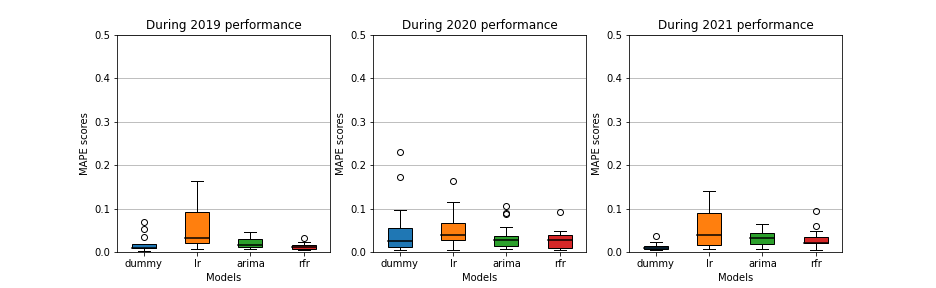
\includegraphics[width=.45\paperwidth]{thesis/images/plots/daily_2019_vs_2020_vs_2021_max_05.png}
%    \caption{Models trained on daily data, split by year, capped at MAPE score <= 0.5}
%    \label{fig:yearplot}
%\end{figure}

\begin{figure}
\centering
\begin{subfigure}[b]{.6\linewidth}
    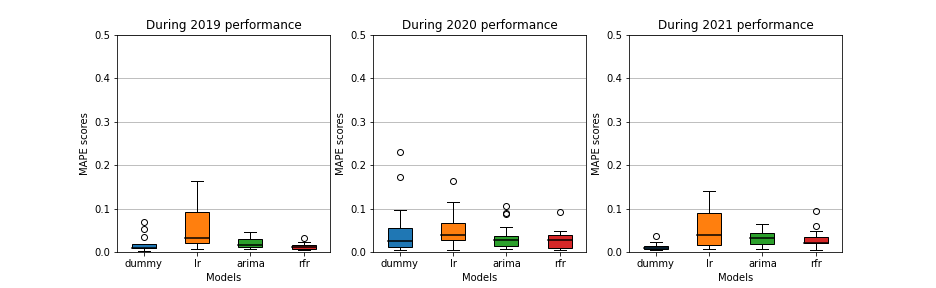
\includegraphics[width=\linewidth]{thesis/images/plots/daily_2019_vs_2020_vs_2021_max_05.png}
    \caption{Models trained on daily data, split by year, capped at MAPE score <= 0.5}
    \label{fig:yearplot}
\end{subfigure}
\begin{subfigure}[b]{.4\linewidth}
    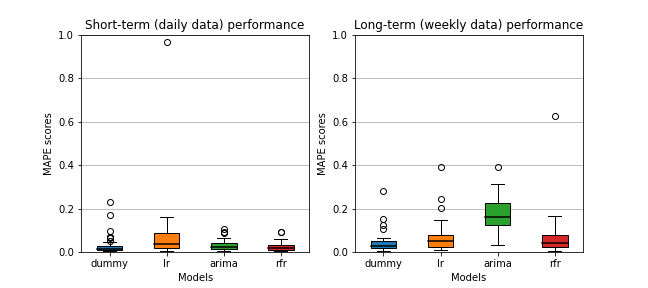
\includegraphics[width=\linewidth]{thesis/images/plots/base_model_comparison_daily_weekly.png}
    \caption{Daily data vs. weekly data}
    \label{fig:modelcompare}
\end{subfigure}
\begin{subfigure}[b]{.4\linewidth}
    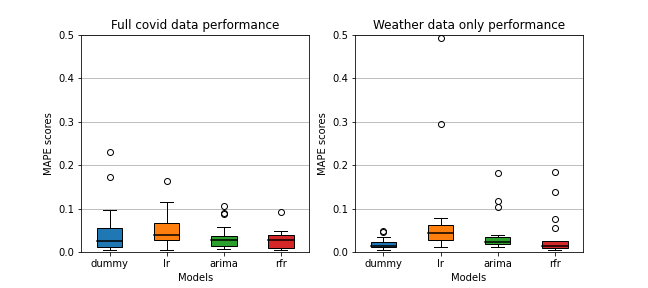
\includegraphics[width=\linewidth]{thesis/images/plots/daily_full_covid_data_vs_weather_data_only_max_05.png}
    \caption{The full dataset vs. weather data only}
    \label{fig:weathervfull}
\end{subfigure}

\begin{subfigure}[b]{.4\linewidth}
    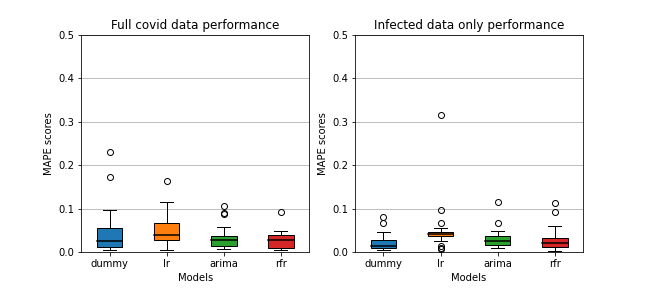
\includegraphics[width=\linewidth]{thesis/images/plots/daily_full_covid_data_vs_infected_data_only_max_05.png}
    \caption{The full dataset vs. COVID-19 infection data only}
    \label{fig:infectvfull}
\end{subfigure} 
\begin{subfigure}[b]{.4\linewidth}
    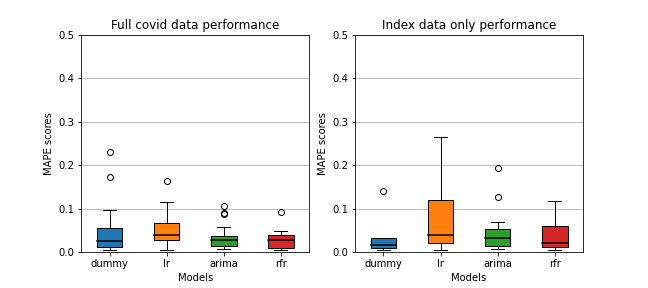
\includegraphics[width=\linewidth]{thesis/images/plots/daily_full_covid_data_vs_index_data_only_max_05.png}
    \caption{The full dataset vs. no additional features}
    \label{fig:indexvfull}
\end{subfigure}
\caption{Comparisons of model scores}
\end{figure}

\subsubsection{Feature performance}
To isolate the impact of data features on our error metric, the same predictions were ran given different selections of features. The results above were given full access to the data, but the following variables were isolated: Weather features, COVID-19- infections, -deaths, -partial/-full vaccinations, stringency of regulations \cite{hale2020variation} and no additional features.
Looking at a comparison of the MAPE scores between weather data only and the full dataset, there is no notable difference in performance (see Figure \ref{fig:weathervfull}). This could indicate that either the weather features are always selected during features selection, or none of the features are of any value to the models.
The latter could be true given none of the models show a notable performance increase from the baseline, but the feature of infections shows that pandemic data does have some influence (see Figure \ref{fig:infectvfull}), at least for the ARIMA and RFR models. The same can be said for deaths, vaccination data and the stringency index, where the ARIMA and RFR model (almost) outperform the baseline model. Although the differences are subtle, they are noticeable, especially compared to LR which shows consistent high error scores compared to the baseline. 
Weather features are the richest of all data and features can be seen as individual features. The only test left is one where the models are given no additional input features and only the response variable defines the output of the models. As a consequence all models increase in performance compared to the baseline as the number of data features decrease, posing the question whether any additional features is helpful at all (see Figure \ref{fig:indexvfull}). 

\begin{table}[h]
\hspace*{\fill}
\parbox{.45\columnwidth}{
\centering
\begin{tabular}{lllll|}
\cline{4-5}
\multicolumn{3}{l|}{}                                                                                                                        & \multicolumn{2}{l|}{\textbf{Baseline compare}} \\ \hline
\multicolumn{1}{|l|}{\textbf{Features}}                    & \multicolumn{1}{l|}{\textbf{Model}} & \multicolumn{1}{l|}{\textbf{MAPE}} & \multicolumn{1}{l|}{\textbf{t-stat}}  & \textbf{p} \\ \hline
\multicolumn{1}{|l|}{\multirow{2}{*}{\textbf{All}}} & \multicolumn{1}{|l|}{\textbf{ARIMA}}                      & 0.0302                                  & -0.3735                               & 0.7096     \\ \cline{2-5} 
\multicolumn{1}{|l|}{}                                       & \multicolumn{1}{|l|}{\textbf{RFR}}                        & 0.0234                                  & 0.6711                                & 0.5037     \\ \hline
\multicolumn{1}{|l|}{\multirow{2}{*}{\textbf{None}}}  & \multicolumn{1}{|l|}{\textbf{ARIMA}}                      & 0.0315                                  & -1.7365                               & 0.0856     \\ \cline{2-5} 
\multicolumn{1}{|l|}{}                                       & \multicolumn{1}{|l|}{\textbf{RFR}}                        & 0.0242                                  & -0.5310                               & 0.5966     \\ \hline
\end{tabular}
\caption{Model MAPE score comparison to baseline, for all dataset features and no additional features}
\label{tbl:modelscores}
}
\hfill
% \end{table}
\parbox{.45\columnwidth}{
\centering
% \begin{table}
\begin{tabular}{l|llll|}
\cline{2-5}
                                        & \multicolumn{1}{l|}{\textbf{Features: All}} & \multicolumn{1}{l|}{\textbf{None}} & \multicolumn{2}{l|}{\textbf{Comparison}}          \\ \hline
\multicolumn{1}{|l|}{\textbf{Model}}    & \multicolumn{1}{l|}{\textbf{MAPE}}    & \multicolumn{1}{l|}{\textbf{MAPE}}   & \multicolumn{1}{l|}{\textbf{t-stat}} & \textbf{p} \\ \hline
\multicolumn{1}{|l|}{\textbf{ARIMA}}    & 0.0341                                     & 0.0434                                    & -0.8300                              & 0.4114     \\ \hline
\multicolumn{1}{|l|}{\textbf{RFR}}      & 0.0300                                     & 0.0408                                    & -0.7865                              & 0.4380     \\ \hline
\multicolumn{1}{|l|}{\textbf{Baseline}} & 0.0475                                     & 0.253                                     & 1.3612                               & 0.1824     \\ \hline
\end{tabular}
\caption{Data feature MAPE score comparison for all the ARIMA, RFR and baseline models}
\label{tbl:datascores}
}
\hspace*{\fill}
\end{table}

\begin{figure}[H]
  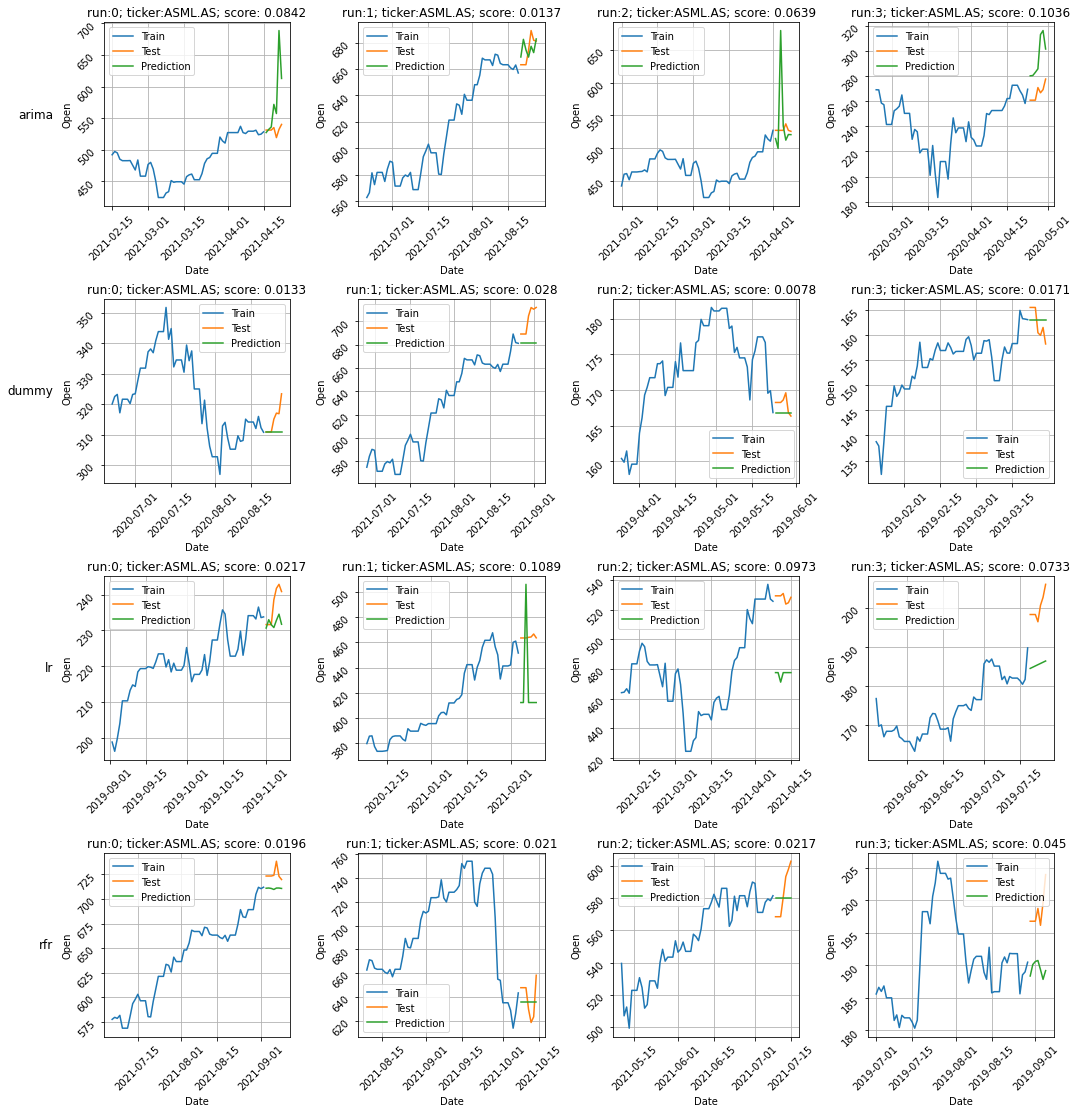
\includegraphics[width=0.9\textwidth]{images/plots/sample_fits_asml.png}
  \caption{Side-by-side model fittings and resulting daily predictions for ASML}
  \label{fig:samplefits}
\end{figure}

\subsection{RQ2: Performance of machine learning techniques in stock market prediction}
As the RFR model is considered as part of the machine learning techniques, it should be compared to the baseline and evaluated on its relative performance. The differences in performance are minute and necessitate an insight into the significance tests to give a reliable measure of difference in performance. For the sake of simplicity, this study has only done this comparison for the daily data, as the weekly data shows unreliable performance. Given a confidence level of 95\% ($\alpha = 0.05$), a T-test on the MAPE scores for the full dataset and the dataset containing no additional features results in the following table \ref{tbl:modelscores}.
With these results it can be said that there is no significant performance difference in using machine learning techniques such as RFR for stock market prediction. The same can be said for the ARIMA model, with the notion that ARIMA does seem to show better performance with reduced features. As each row in table \ref{tbl:modelscores} refers to an individual T-test, the dimensions can also be flipped to test whether the features in the data influence the models in table \ref{tbl:datascores}.
This research shows there is no significant difference in the mean MAPE error scores between all or no additional features in the data, for none of the models.
\section{Discussion}
\label{sec:dis}
When viewing the results compared to the baseline model, better performance was to be expected from the ARIMA and RFR models. These models should have been able to capture the variance of the non-linear time-series, when properly tuned and fitted. The additional features presented by the COVID-19 pandemic do seem to sporadically add accuracy, however the significance tests show that these are most likely a random or coincidental occurrence rather than a relationship in the data. Linear regression actually consistently performed worse than the baseline, which indicates that the data is non-linear.
In light of related work, this could be due to the methodology of automated model fitting and tuning. Previous studies of forecasting models generally approach these tasks as an iterative process, where a single model is developed on very specific data with large amounts of manual tuning. In these results large parts of the test scores already needed to be discarded due to obvious fitting errors caused by noise in the data, preprocessing or failures of the code. Where EDA showed there was potential in the data and models, when implemented on a larger scale it shows that without manual intervention, these models do not generalize. This was somewhat expected, as other related work already showed that stock market prediction relies on domain knowledge or technical analysis. % The EMH states that with asset prices reflecting all available information, there is no possible way of outperforming the market as asset prices only react to new information. 
As the COVID-19 pandemic was new information at the end of 2019, there was a consequential dip in oil futures and related assets, which set the precedent of the pandemic becoming old information. Also it was clear that this dip in oil futures was a result of compounding events rather than just an effect of the pandemic. Another possible explanation for the insignificant results is that there is no causal relationship between our features. Although publicly available data could've influenced the behavioural psychology of traders, this is a relationship primarily determined by the traders' psychology and only has a secondary relation to this study's data. As businesses moved to working remotely from their employees homes, lockdown effects were overcome for most industries and the effect on the economy was consequently negated. Along with quick developments in vaccines, this could've led traders to the conclusion that the pandemic was of little importance after the first wave of infections. These developments were mostly covered in news stories, which are difficult to quantify, but are generally the main source of information for traders. Any relationship with pandemic information is probably only visible on long term analysis, where events on the stock market accumulate over time and variance decreases.
Although technology has come a long way, and SOTA machine learning models have shown promise in varying fields of expertise, it is clear that these models do not learn 'automatically'. A lot of expertise is needed to properly fit and tune a model to very specific data and only then can it be considered as a viable solution for the specific problem in mind. Generalization of models is acquired by training with large amounts of data, but only when the model in question can do the same on very specific data. For instance, models that perform character recognition in images can generalize to other tasks, such as object classification, however this comes with complex engineering of the models and large amounts of prepared data. In this case, the EDA showed promise on prediction models combined with pandemic data. And with large amounts of fitting, tuning and engineering of a single model it might still be possible to achieve a significant result. Still, generalization of such models comes with large volumes of data and preparation, and only when a precedent is set research can work towards a more general solution. In this research experiments were performed with different models, such as Xgboost, but from sample fittings it was clear it would not outperform RFR without additional data or proper manual tuning.

\section{Conclusions}
\label{sec:conc}
Summarizing the results and discussion, this study can not confirm there is any added benefit of including COVID-19 pandemic data as a explanatory variable for the purpose of stock market predictions. Considering the individual contributions of environmental factors, such as weather, this study can not establish a significant relationship. The same is applicable for any of the individual COVID-19 pandemic features, where it is concluded that any relation is either coincidental or inconclusive as no significant performance difference can be measured.
This does not mean there is no added benefit of applying SOTA machine learning techniques or models to improve prediction accuracy, as indicated by related work. This study could not establish a significant relationship between pandemic data and stock market values with ARIMA or RFR models, especially compared to the performance of the baseline model. Forming a basis for more complex models, such as LSTM/RNN, is therefore unsustainable as this study can not provide the data these models require to achieve significant results. There remains a possibility for pre-trained models or transfer learning to improve results, however this would require further research to verify. Financial theories debate on whether an algorithm can consistently beat (the majority of) the stock market and as a consequence one can imagine these models are not within the grasp of the general public. Within the scope of this research it is concluded that it is not possible to achieve such a result and leave this as a springboard for further research.
Although this study did not establish a statistical significant result, there is anecdotal evidence of an impact during the first infection wave of the COVID-19 pandemic. With purpose built models and data there is a possibility of constructing accurate time-series forecasts, but this comes at the cost of generalization.

%%
%% The acknowledgments section is defined using the "acks" environment
%% (and NOT an unnumbered section). This ensures the proper
%% identification of the section in the article metadata, and the
%% consistent spelling of the heading.
% \begin{acks}
% The researcher(s) would like to thank the external and internal supervisors Dr. Julian Antonio Pucheta and Dr. Christian Rodriguez Rivero for supporting this research. As the COVID-19 pandemic is still ongoing as of writing (December 2021), it is a trying time for everyone to keep working. And in that light thanks are given to the University of Amsterdam for their patience and support. 
% Finally I, Maarten Peters, would personally like to acknowledge my partner Melissa van der Werf for supporting me during my two year part-time masters at the University of Amsterdam. As my advisors at the university told, a part-time study next to a full-time employment is no trivial matter, but I can recommend it to anybody who is willing to invest their time in developing their own knowledge and skills, as the effort is well worth the result.
% \end{acks}

%%
%% The next two lines define the bibliography style to be used, and
%% the bibliography file.
\bibliographystyle{ACM-Reference-Format}
\bibliography{thesis/0_literature.bib}


\end{document}
\endinput